\DiaryEntry{All-Pairs Shortest Path Algorithms - Floyd-Warshall Algorithm}{2020-05-25}{Algorithms}

In this entry we consider the Floyd-Warshal algorithm, which is another way to solve the all-pairs shortest path problem.

We denote by $d_{i,j}^{(k)}$ the weight of the shortest path from vertex $i$ to $j$ for which all intermediate vertices are in the set $1,2,\ldots,k$. When $k=0$, the path from vertex $i$ to $j$ has no intermediate vertices at all; therefore the path has one edge and therefore $d_{i,j}^{(0)} = w_{i,j}$.  For longer paths we have the following recursion (proof omitted)

\bee
d_{i,j}^{(k)} = \begin{cases} w_{i,j} & \quad k=0 \\
  \min \left( d^{(k-1)}_{i,j}, d^{(k-1)}_{i,k} + d^{(k-1)}_{k,j}  \right) & \quad k \geq 1
  \end{cases}
\eee

For any path, all intermediate vertices are in the set $\{1,2,\ldots,n\}$; therefore the final result is $d^{(n)}_{i,j} = \delta(i,j)$. We can collect these values in a matrix $\Dbf^{(n)}$.

From an intuitive point of view, we compare the weigh of the existing path $d_{i,j}^{(k)}$ with the weight of a path from vertex $i$ to $k$ and a path from vertex $k$ to $i$. Only if the latter is better, we update the weight.


\paragraph{Algorithm Definition.} The algorithm is contained in the following pseudo-code.

\begin{Verbatim}[numbers=left, xleftmargin=5mm]
FLoyd-Warshal(W)
   n = W.rows
   D(0) = W
   for k = 1 to n
      D(k) = zero(n,n)
      for i = 1 to n
         for j = 1 to n
            d(i,j,k) = min(d(i,j,k-1), d(i,k,k-1) + d(k,j,k-1))
   return D(n)
\end{Verbatim}


\paragraph{Shortest Path Construction.} We consider calculating the predecessor matrix within the above algorithm. Specifically, we compute a sequence of predecesor matrices \\ $\Pi^{(0)}, \Pi^{(1)}, \ldots, \Pi^{(n)}$ and define $\pi_{i,j}^{(k)}$ as predecessor of veretx $j$ on a shortest path from $i$ with all intermediate vertices in the set $\{1,2,\ldots,k\}$. We therefore have

\be\label{eq:apsp_1}
\pi_{i,j}^{(k)} = \begin{cases} -1 & \text{if } i=j \text{ or } w_{i,j} = \infty \\
  i & \text{if } i \neq j \text{ or } w_{i,j} < \infty \end{cases}
\ee

For recursion, we use

\bee
\pi_{i,j}^{(k)} = \begin{cases} \pi_{i,j}^{(k-1)} & \text{if } d^{(k-1)}_{i,j} \leq d^{(k-1)}_{i,k} + d^{(k-1)}_{k,j} \\
  \pi_{k,j}^{(k-1)} & \text{if } d^{(k-1)}_{i,j} > d^{(k-1)}_{i,k} + d^{(k-1)}_{k,j}
  \end{cases}
\eee


We can incorporate this into the above algorithm and calculate minimum weights and construct the corresponding shortest paths using the following algorithm.

\begin{Verbatim}[numbers=left, xleftmargin=5mm]
FLoyd-Warshal(W)
   n = W.rows
   D(0) = W
   pi(0)= init-pi(W)
   for k = 1 to n
      D(k) = zero(n,n)
      for i = 1 to n
         for j = 1 to n
            if d(i,j,k-1) <= d(i,k,k-1) + d(k,j,k-1)
               d(i,j,k) = d(i,j,k-1)
               pi(i,j,k) = pi(i,j,k-1)
            else
               d(i,j,k) = d(i,k,k-1) + d(k,j,k-1)
               pi(i,j,k) = pi(k,j,k-1)
            end
   return D(n), Pi(n)
\end{Verbatim}

In this pseudo-code, the procedure \verb init-pi(W)  initializes $\Pi^{(0)}$ according to \eqref{eq:apsp_1}.


\paragraph{Example.} We execute the Floyd-Warshal algorithm on the example graph from the previous entry.

\begin{figure}[H]v
\centering
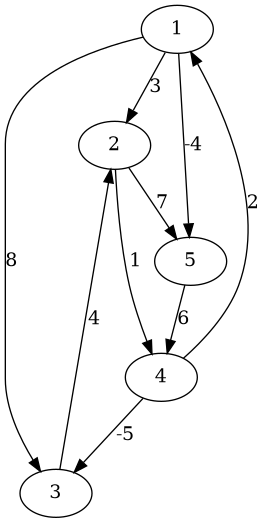
\includegraphics[scale=0.5]{images/apsp_01.png}
\end{figure}

The corresponding matrices $\Wbf$ and $\Pi^{(0)}$ have the following structure

\bee
\Wbf = \begin{pmatrix} 0 & 3 & 8 & \infty & -4 \\
  \infty & 0 & \infty & 1 & 7 \\
  \infty & 4 & 0 & \infty & \infty \\
  2 & \infty & -5 & 0 & \infty \\
  \infty & \infty & \infty & 6 & 0
\end{pmatrix},
\quad
\Pi^{(0)} = \begin{pmatrix} -1 & 1 & 1 & -1 & 1 \\
  -1 & -1 & -1 & 2 & 2 \\
  -1 & 3 & -1 & -1 & -1 \\
  4 & -1 & 4 & -1 & -1 \\
  -1 & -1 & -1 & 5 & -1
\end{pmatrix}
\eee

After the first iteration, the algorithm has considered paths of up to length $2$. We have the following matrices (entries modified in this iteration are shown in boxes)

\bee
\Dbf^{(1)} = \begin{pmatrix} 0 & 3 & 8 & \infty & -4 \\
  \infty & 0 & \infty & 1 & 7 \\
  \infty & 4 & 0 & \infty & \infty \\
  2 & \boxed{5} & -5 & 0 & \boxed{-2} \\
  \infty & \infty & \infty & 6 & 0
\end{pmatrix},
\quad
\Pi^{(1)} = \begin{pmatrix} -1 & 1 & 1 & -1 & 1 \\
  -1 & -1 & -1 & 2 & 2 \\
  -1 & 3 & -1 & -1 & -1 \\
  4 & \boxed{1} & 4 & -1 & \boxed{1} \\
  -1 & -1 & -1 & 5 & -1
\end{pmatrix}
\eee

The algorithm has found a path from vertex $4$ to $2$ with weight $\Dbf^{(1)}_{4,2} = 5$. We can use the $4$-th row of $\Pi^{(1)}$ to obtain the path between the two vertices (we use the procedure \verb Print-All-Pairs-Shortest-Paths(Pi,i,j)  for this): $\Pi^{(1)}_{4,2} = 1$ and $\Pi^{(1)}_{4,1} = 4$ so the path is $4-1-2$. Subsequent iterations yield more / shorter paths; the final result is given by

\bee
\Dbf^{(5)} = \begin{pmatrix} 0 & 1 & -3 & 2 & -4 \\
  3 & 0 & -4 & 1 & -1 \\
  7 & 4 & 0 & 5 & 3 \\
  2 & -1 & -5 & 0 & -2 \\
  8 & 5 & 1 & 6 & 0
\end{pmatrix},
\quad
\Pi^{(5)} = \begin{pmatrix} -1 & 3 & 4 & 5 & 1 \\
  4 & -1 & 4 & 2 & 1 \\
  4 & 3 & -1 & 2 & 1 \\
  4 & 3 & 4 & -1 & 1 \\
  4 & 3 & 4 & 5 & -1
\end{pmatrix}
\eee

All observations from previous journal entry (values of $\infty$ disappearing and path weights decreasing with subsequent iterations) are still valid.



%%% Local Variables:
%%% mode: latex
%%% TeX-master: "journal"
%%% End:
